\documentclass[11pt,a4paper]{article}

\usepackage{mathpazo}
\usepackage{url}
\usepackage{verbatim}

\usepackage{tikz}
\usetikzlibrary{calc, external, intersections, through}
\tikzexternalize[prefix=tikz/]

\textwidth=15cm
\textheight=23cm
\topmargin=12pt
\headheight=0pt
\oddsidemargin=1em
\headsep=0pt
\renewcommand{\baselinestretch}{1.1}
\setlength{\parskip}{0.2\baselineskip plus 1pt minus 1pt}
\parindent=0pt

\renewcommand{\arraystretch}{1.3}

\begin{document}
\thispagestyle{empty}


\begin{center}
\textbf{\LARGE How to Do Trigonometry Without\\\medskip
Memorizing (Almost) Anything}

\bigskip
\bigskip

\textbf{\Large Moti Ben-Ari}

\medskip

Weizmann Institute of Science

\url{http://www.weizmann.ac.il/sci-tea/benari/}
\end{center}

{\footnotesize \copyright{}\  2017 by Moti Ben-Ari. This work is licensed under the Creative Commons Attribution-ShareAlike 3.0 Unported License. To view a copy of this license, visit \url{http://creativecommons.org/licenses/by-sa/3.0/} or send a letter to Creative Commons, 444 Castro Street, Suite 900, Mountain View, California, 94041.}

\begin{center}
\includegraphics[width=.2\textwidth]{../by-sa.png}
\end{center}


\bigskip

I would like to thank Avital Elbaum Cohen and Ronit Ben-Bassat Levy for their helpful comments.

\bigskip

Trigonometry facilitates geometric reasoning using algebraic computation. To the student trigonometry can appear as a large set of obscure formulas to be memorized. The purpose of this document is to show that trigonometric identities can be obtained by geometric reasoning with little memorization.

The appendices contains proofs of the law of sines and the law of cosines. Although these formulas are easy to memorize, it is useful to see how they can be proved using only geometric facts.

%%%%%%%%%%%%%%%%%%%%%%%%%%%%%%%%%%%%%%%%%%%%%%%%%%%%%%%%%%%%%%%

\section{Basic definitions}

We have to start with definitions that must be memorized. In a right triangle:
\begin{center}
% Right triangles
\begin{tikzpicture}[scale=4]
% Outer triangle
\coordinate (origin1) at (0,0);
% Draw ray at 30
\draw[rotate=30] (origin1) node [above right,xshift=26pt,yshift=1pt] {$\theta$} -- node [above] {$c$} +(1.4,0) coordinate (point1);
% Drop altitude from end of ray
\draw (point1) -- node [right] {$a$}  (point1 |- origin1) coordinate (altitude1);
% Connect origin to altitude
\draw (origin1) -- node [below] {$b$} (altitude1);
% Square for right angle
\draw (altitude1) rectangle +(-1pt,1pt);
\end{tikzpicture}
\end{center}
the sine and cosine of an angle are defined as the ratios of the sides of the triangle with the hypotenuse:\footnote{This document does not discuss the tangent. Since $\tan\theta = \sin\theta/\cos\theta$, identities for tangent can be obtained from those for sine and cosine.}
\[
\sin \theta = \frac{a}{c},\;\; \cos\theta = \frac{b}{c}\,.
\]
The ratios can be verbally expressed as ``sine is opposite over hypotenuse'' and ``cosine is adjacent over hypotenuse.''

The trigonometric functions are functions of the angle alone and do not depend on the size of the triangle. Given two right triangles with the same angles:
\begin{center}
% Nested right triangles
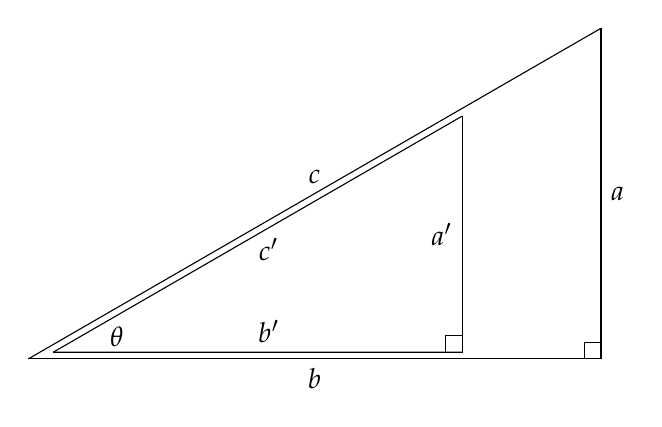
\begin{tikzpicture}[scale=6]
% Outer triangle
\coordinate (origin1) at (0,0);
% Draw ray at 30
\draw[rotate=30] (origin1) node [above right,xshift=26pt,yshift=1pt] {$\theta$} -- node [above] {$c$} +(1.4,0) coordinate (point1);
% Drop altitude from end of ray
\draw (point1) -- node [right] {$a$}  (point1 |- origin1) coordinate (altitude1);
% Connect origin to altitude
\draw (origin1) -- node [below] {$b$} (altitude1);
% Square for right angle
\draw (altitude1) rectangle +(-1pt,1pt);
% Inner triangle slightly offset from (0,0)
\coordinate (origin2) at (1.5pt,.4pt);
% Draw ray at 30
\draw[rotate=30] (origin2) -- node [below,xshift=4pt,yshift=2pt] {$c'$} +(1,0) coordinate (point2);
% Drop altitude from end of ray
\draw (point2) -- node [left] {$a'$} (point2 |- origin2) coordinate (altitude2);
% Connect origin to altitude
\draw (origin2) -- node [above,xshift=4pt] {$b'$} (altitude2);
% Square for right angle
\draw (altitude2) rectangle +(-1pt,1pt);
\end{tikzpicture}
\end{center}
the similarity of the triangles gives:
\[
\frac{c'}{c} = \frac{a'}{a} = \frac{b'}{b}\,,
\]
and then:
\[
\frac{a}{c} = \frac{a'}{c'} = \sin \theta
\]

\[
\frac{b}{c} = \frac{b'}{c'} = \cos \theta\,.
\]

Since we are free to choose the length of one of the sides, it will make our lives easier if we choose the length of the hypotenuse to be $1$:
\begin{center}
% Right triangles with hypotenuse 1
\begin{tikzpicture}[scale=4]
% Outer triangle
\coordinate (origin1) at (0,0);
% Draw ray at 30
\draw[rotate=30] (origin1) node [above right,xshift=26pt,yshift=1pt] {$\theta$} -- node [above] {$1$} +(1.4,0) coordinate (point1);
% Drop altitude from end of ray
\draw (point1) -- node [right] {$\sin \theta$}  (point1 |- origin1) coordinate (altitude1);
% Connect origin to altitude
\draw (origin1) -- node [below] {$\cos \theta$} (altitude1);
% Square for right angle
\draw (altitude1) rectangle +(-1pt,1pt);
\end{tikzpicture}
\end{center}
Therefore, the denominator of the sine and cosine ratios is $1$ and can be ignored. The functions $\sin\theta$ and $\cos\theta$ give the lengths of the opposite and adjacent sides of the triangle. From Pythagoras's theorem we have:
\[
\sin^2\theta + \cos^2\theta = 1^2 = 1
\]

%%%%%%%%%%%%%%%%%%%%%%%%%%%%%%%%%%%%%%%%%%%%%%%%%%%%%%%%%%%%%%%

\section{The unit circle}

By taking the hypotenuse of the right angle to be $1$, we can transform the entire presentation of trigonometry into the \emph{unit circle} in the coordinate system of the plane. The values $\cos\theta$ and $\sin\theta$ are not only the lengths of the sides of the triangle, but also the coordinates $(\cos\theta,\sin\theta)$ of the intersection of the ray from the origin with the unit circle:
\begin{center}
% The unit circle
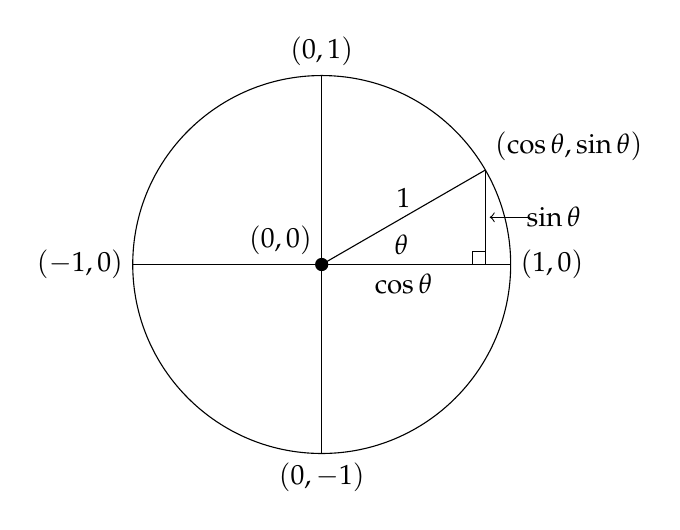
\begin{tikzpicture}[scale=2.4]
\coordinate (origin) at (0,0);
% Draw circle
\draw[name path=circle] (origin) node [above left] {$(0,0)$} circle [radius=1];
% Draw axes
\draw[name path=x] (-1,0) node [left] {$(-1,0)$} -- (1,0) node [right] {$(1,0)$};
\draw (0,-1) node [below] {$(0,-1)$} -- (0,1) node [above] {$(0,1)$};
% Draw ray
\draw[rotate=30,name path=ray] (origin) node [above right,xshift=8mm] {$\theta$} -- node [above] {$1$} (1,0);
% Get intersection of circle and ray
\path [name intersections={of=circle and ray, by=on-circle}];
% Draw altitude from intersection to x-axis
\draw[name path=altitude] (on-circle) node[above right] {$(\cos\theta,\sin\theta)$} -- node [right,xshift=4mm] {$\sin \theta$} (on-circle |- origin);
\draw[->] (1.1,.25) -- +(-6pt,0);
% Get intersection of altitude and x-axis
\path [name intersections={of=altitude and x, by=on-x}] (origin) -- node [below] {$\cos \theta$} (on-x);
% Square for right angle at intersection
\draw (on-x) rectangle +(-2pt,2pt);
% Dot at origin
\fill (origin) circle [radius=1pt];
\end{tikzpicture}
\end{center}

The unit of angles is the \emph{degree}. In a circle, angles are measured starting from the positive $x$-axis, counterclockwise for positive angles and clockwise for negative angles. There are $360$ degrees in a circle (notation $360^\circ$). The axes of the Cartesian coordinate system naturally divide the unit circle into four \emph{quadrants}:
\begin{center}
% The unit circle with main axes
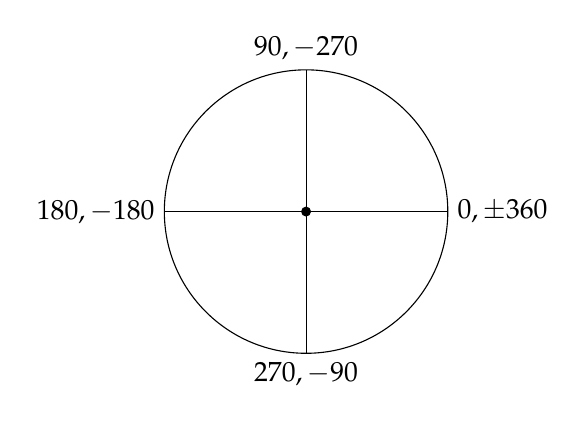
\begin{tikzpicture}[scale=1.8]
\coordinate (origin) at (0,0);
% Draw circle
\draw (origin) circle [radius=1];
% Draw axes
\draw (-1,0) node [left] {$180,-180$} -- (1,0) node [right] {$0,\pm 360$};
\draw (0,-1) node [below] {$270,-90$} -- (0,1) node [above] {$90,-270$};
% Dot at origin
\fill (origin) circle [radius=1pt];
\end{tikzpicture}
\end{center}

An alternate unit of angles is the \emph{radian}. One radian is the angle that subtends an arc on a circle whose length is equal to the radius. Since the radius of the unit circle is $1$, its circumference is of length $2\pi$, and as a ray traces out the entire circumference (counterclockwise) it moves from an angle of $0$ radians to an angle of $2\pi$ radians:
\begin{center}
% The unit circle with main axes
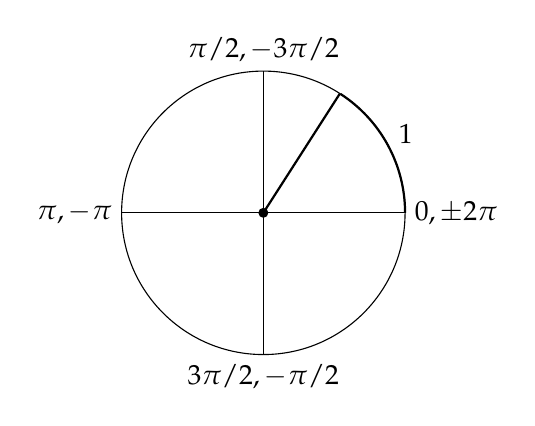
\begin{tikzpicture}[scale=1.8]
\coordinate (origin) at (0,0);
% Draw circle
\draw (origin) circle [radius=1];
% Draw axes
\draw (-1,0) node [left] {$\pi,-\pi$} -- (1,0) node [right] {$0,\pm 2\pi$};
\draw (0,-1) node [below] {$3\pi/2,-\pi/2$} -- (0,1) node [above] {$\pi/2,-3\pi/2$};
% Draw one radian
\draw[thick] (origin) -- (57.3:1);
\draw[thick]  (1,0) arc(0:57:1);
\node at (29:1.15) {$1$};
% Dot at origin
\fill (origin) circle [radius=1pt];
\end{tikzpicture}
\end{center}
One radian equals approximately $57.3$ degrees.

From the coordinates of the intersection of the $x$- and $y$-axes with the unit circle, we can read off the values of sine and cosine for these angles:
\begin{displaymath}
\renewcommand{\arraystretch}{1.2}
\begin{array}{|c|c|c|c|}
\hline
\textrm{Angle} & \textrm{Angle} & \sin & \cos\\
\textrm{(degrees)} & \textrm{(radians)} & & \\\hline
0 & 0 & 0 & 1\\\hline
90 & \pi/2 & 1 & 0\\\hline
180 & \pi & 0 & -1\\\hline
270 & 3\pi/2 & -1 & 0\\
\hline
\end{array}
\end{displaymath}

%%%%%%%%%%%%%%%%%%%%%%%%%%%%%%%%%%%%%%%%%%%%%%%%%%%%%%%%%%%%%%%

\section{Dividing the unit circle into $8$ segments}

We have seen that the axes divide the unit circle into $4$ quadrants. It is useful to divide the unit circle into $6$, $8$ and $12$ segments, and to learn the sine and cosine of the corresponding angles. First, divide each quadrant in half to produce $8$ segments, where the angle of each segment is $45^\circ$ or $\pi/4$ radians:

\begin{center}
% The unit circle divided into 45 degree segments
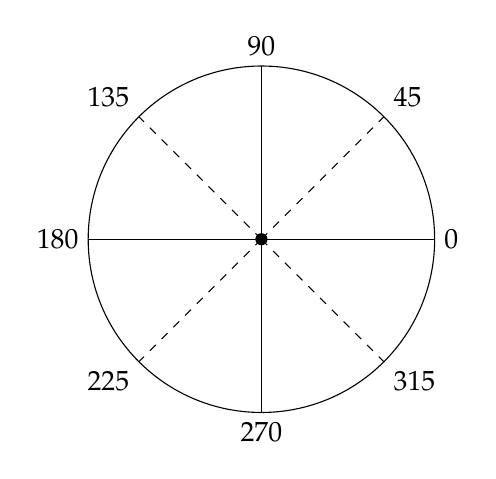
\begin{tikzpicture}[scale=2.2]
\coordinate (origin) at (0,0);
% Draw circle
\draw (origin) circle [radius=1];
% Draw axes
\draw (-1,0) node [left] {$180$} -- (1,0) node [right] {$0$};
\draw (0,-1) node [below] {$270$} -- (0,1) node [above] {$90$};
% Draw other angles
\draw[dashed] (origin) -- +(45:1) node[above right] {$45$};
\draw[dashed] (origin) -- +(135:1) node[above left] {$135$};
\draw[dashed] (origin) -- +(225:1) node[below left] {$225$};
\draw[dashed] (origin) -- +(315:1) node[below right] {$315$};
% Dot at origin
\fill (origin) circle [radius=1pt];
\end{tikzpicture}
\hspace{5em}
% The unit circle with radians divided into pi/4 segments
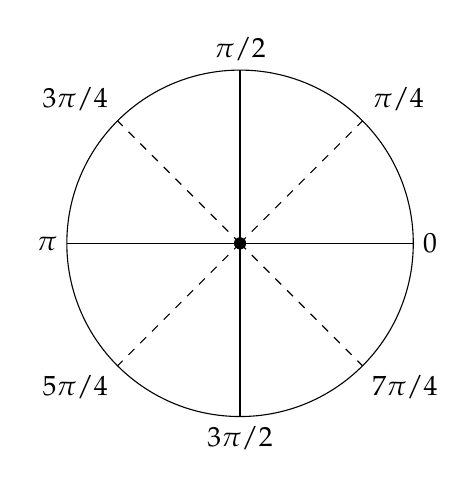
\begin{tikzpicture}[scale=2.2]
\coordinate (origin) at (0,0);
% Draw circle
\draw (origin) circle [radius=1];
% Draw axes
\draw (-1,0) node [left] {$\pi$} -- (1,0) node [right] {$0$};
\draw (0,-1) node [below] {$3\pi/2$} -- (0,1) node [above] {$\pi/2$};
% Draw other angles
\draw[dashed] (origin) -- +(45:1) node[above right] {$\pi/4$};
\draw[dashed] (origin) -- +(135:1) node[above left] {$3\pi/4$};
\draw[dashed] (origin) -- +(225:1) node[below left] {$5\pi/4$};
\draw[dashed] (origin) -- +(315:1) node[below right] {$7\pi/4$};
% Dot at origin
\fill (origin) circle [radius=1pt];
\end{tikzpicture}
\end{center}

What are the sine and cosine of $45^\circ$? In the triangle:
\begin{center}
% Right triangle with 45 degree angles
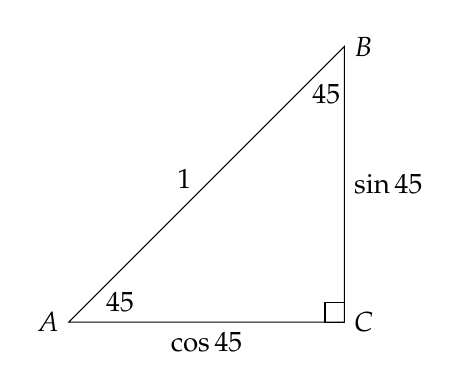
\begin{tikzpicture}[scale=3.5]
% Coordinates
\coordinate (origin) at (0,0);
\coordinate (lower-right) at (1,0);
\coordinate (upper-right) at (1,1);
% Draw triangle
\draw (origin) node[left] {$A$} node[above right,xshift=10pt] {$45$} -- node[below] {$\cos 45$} (lower-right) node[right] {$C$} -- node[right] {$\sin 45$} (upper-right) node[right] {$B$} node[below left,xshift=2pt,yshift=-10pt] {$45$} -- node[left,xshift=-2pt,yshift=2pt] {$1$} cycle;
% Square for right angle
\draw (lower-right) rectangle +(-2pt,2pt);
\end{tikzpicture}
\end{center}
If the angle $\angle BAC$ is $45^\circ$, the opposite angle $\angle ABC$ must also be $45^\circ$ so that the sum of the angles in the triangle is $180^\circ$. The triangle is isoceles so the sine and the cosine are equal. By Pythagoras's theorem:
\begin{eqnarray*}
\sin^2 45 + \cos^2 45 &=& 1\\
2\sin^2 45 &=& 1\\
\sin 45 &=& \frac{1}{\sqrt{2}} = \frac{1}{\sqrt{2}}\cdot \frac{2}{2} =\frac{\sqrt{2}}{2}\\
\cos 45 &=& \sin 45 = \frac{\sqrt{2}}{2}\,.
\end{eqnarray*}

%%%%%%%%%%%%%%%%%%%%%%%%%%%%%%%%%%%%%%%%%%%%%%%%%%%%%%%%%%%%%%%

\section{The sine and cosine of angles greater than $90^\circ$}

Now that we know the sine and cosine of $45^\circ$, we can ask about the other three symmetrical angles $135^\circ$, $225^\circ$, $315^\circ$. With the help of our friend the unit circle, we can immediately find their sine and cosine.

We first do so for an arbitrary angle $\theta$ in the first quadrant. Since the projections of the rays on the $x$- and $y$-axes are the same, we only have to change the sign of the result. For the second quadrant:
\begin{center}
% Functions of 180-\theta
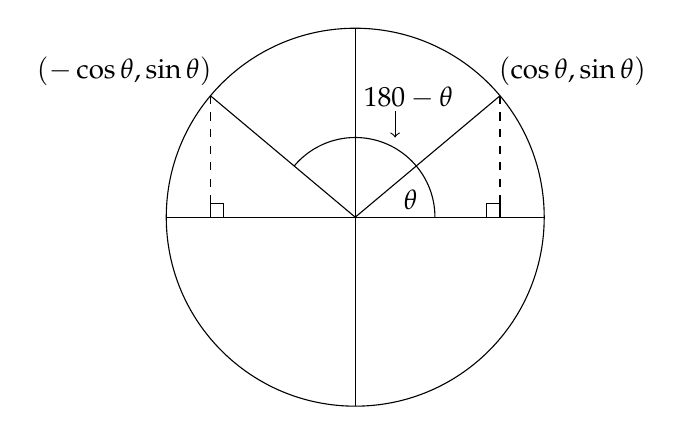
\begin{tikzpicture}[scale=2.4]
\coordinate (origin) at (0,0);
% Draw circle
\draw[name path=circle] (origin) circle [radius=1];
% Draw axes
\draw (-1,0) -- (1,0);
\draw (0,-1) -- (0,1);
% Draw first ray
\path[name path=ray1] (origin) -- +(40:1.1);
\path[name intersections={of=circle and ray1,by=on-circle1}];
\draw (origin) node[above right,xshift=14pt,yshift=-1pt] {$\theta$} -- (on-circle1) node[above right,xshift=-4pt] {$(\cos \theta, \sin \theta)$};
% Draw altitude and square for right angle
\draw[dashed] (on-circle1) -- (on-circle1 |- origin);
\draw (on-circle1 |- origin) rectangle +(-2pt,2pt);
% Draw second ray
\path[name path=ray2] (origin) -- +(140:1.1);
\path[name intersections={of=circle and ray2,by=on-circle2}];
\draw (origin) -- (on-circle2) node[above left,xshift=4pt] {$(-\cos \theta, \sin \theta)$};
% Draw altitude and square for right angle
\draw[dashed] (on-circle2) -- (on-circle2 |- origin);
\draw (on-circle2 |- origin) rectangle +(2pt,2pt);
% Draw the arc for 180-\theta
\draw (12pt,0) arc(0:140:12pt);
\node at (8pt,18pt) {$180-\theta$};
\draw[->] (6pt,16pt) -- +(0,-4pt);
\end{tikzpicture}
\end{center}
so:
\[
\begin{array}{l}
\cos 135=\cos (180-45)= -\cos 45= \displaystyle -\frac{\sqrt{2}}{2}\\
\sin 135=\sin (180-45)= \sin 45= \displaystyle \frac{\sqrt{2}}{2}\,.
\end{array}
\]
For the third quadrant:
\begin{center}
% Functions of 180+\theta
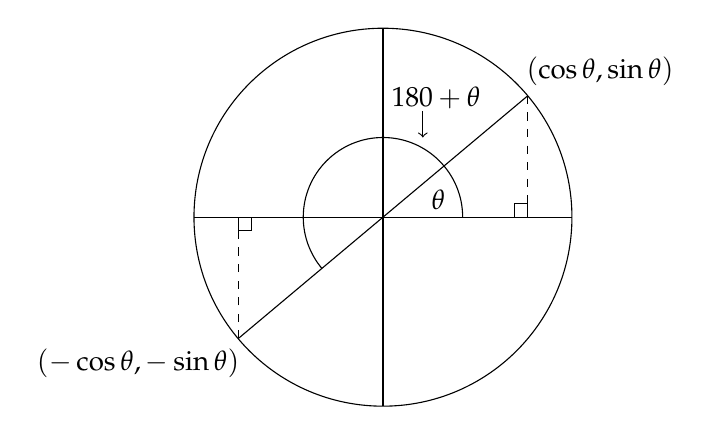
\begin{tikzpicture}[scale=2.4]
\coordinate (origin) at (0,0);
% Draw circle
\draw[name path=circle] (origin) circle [radius=1];
% Draw axes
\draw (-1,0) -- (1,0);
\draw (0,-1) -- (0,1);
% Draw first ray
\path[name path=ray1] (origin) -- +(40:1.1);
\path[name intersections={of=circle and ray1,by=on-circle1}];
\draw (origin) node[above right,xshift=14pt,yshift=-1pt] {$\theta$} -- (on-circle1) node[above right,xshift=-4pt] {$(\cos \theta, \sin \theta)$};
% Draw altitude and square for right angle
\draw[dashed] (on-circle1) -- (on-circle1 |- origin);
\draw (on-circle1 |- origin) rectangle +(-2pt,2pt);
% Draw second ray
\path[name path=ray2] (origin) -- +(-140:1.1);
\path[name intersections={of=circle and ray2,by=on-circle2}];
\draw (origin) -- (on-circle2) node[below left,xshift=4pt] {$(-\cos \theta, -\sin \theta)$};
% Draw altitude and square for right angle
\draw[dashed] (on-circle2) -- (on-circle2 |- origin);
\draw (on-circle2 |- origin) rectangle +(2pt,-2pt);
% Draw the arc for 180+\theta
\draw (12pt,0) arc(0:220:12pt);
\node at (8pt,18pt) {$180+\theta$};
\draw[->] (6pt,16pt) -- +(0,-4pt);
\end{tikzpicture}
\end{center}
\[
\begin{array}{l}
\cos 225 =\cos (180+45)= -\cos 45= \displaystyle -\frac{\sqrt{2}}{2}\\
\sin 225 =\sin (180+45)= -\sin 45= \displaystyle -\frac{\sqrt{2}}{2}\,.
\end{array}
\]
For the fourth quadrant, it convenient to use the negative angle $-\theta$ instead of the positive angle $360-\theta$:
\begin{center}
% Functions of -\theta
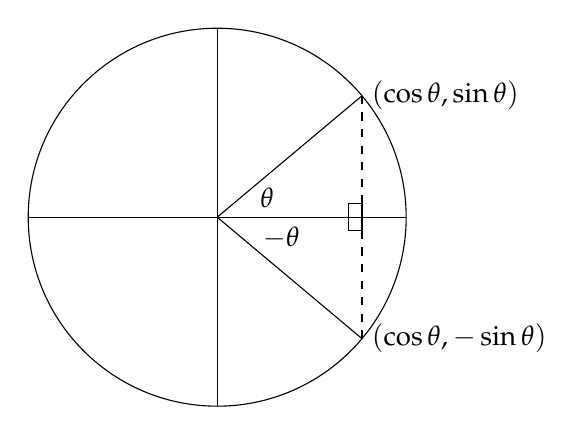
\begin{tikzpicture}[scale=2.4]
\coordinate (origin) at (0,0);
% Draw circle
\draw[name path=circle] (origin) circle [radius=1];
% Draw axes
\draw (-1,0) -- (1,0);
\draw (0,-1) -- (0,1);
% Draw first ray
\path[name path=ray1] (origin) -- +(40:1.1);
\path[name intersections={of=circle and ray1,by=on-circle1}];
\draw (origin) node[above right,xshift=12pt] {$\theta$} -- (on-circle1) node[right] {$(\cos \theta, \sin \theta)$};
% Draw altitude and square for right angle
\draw[dashed] (on-circle1) -- (on-circle1 |- origin);
\draw (on-circle1 |- origin) rectangle +(-2pt,2pt);
% Draw second ray
\path[name path=ray2] (origin) -- +(-40:1.1);
\path[name intersections={of=circle and ray2,by=on-circle2}];
\draw (origin) node[below right,xshift=13pt] {$-\theta$} -- (on-circle2) node[right] {$(\cos \theta, -\sin \theta)$};
% Draw altitude and square for right angle
\draw[dashed] (on-circle2) -- (on-circle2 |- origin);
\draw (on-circle2 |- origin) rectangle +(-2pt,-2pt);
\end{tikzpicture}
\end{center}
\[
\begin{array}{l}
\cos 315=\cos (-45)= \cos 45= \displaystyle \frac{\sqrt{2}}{2}\\
\sin 315=\sin (-45)= -\sin 45= \displaystyle -\frac{\sqrt{2}}{2}\,.
\end{array}
\]
Summarizing the results in a table:
\begin{displaymath}
\renewcommand{\arraystretch}{1.3}
\begin{array}{|c|c|c|c|}
\hline
\textrm{Angle} & \textrm{Angle} & \sin & \cos\\
\textrm{(degrees)} & \textrm{(radians)} & & \\\hline
\theta& \theta&  \sin\theta &  \cos\theta \\\hline
180-\theta& \pi - \theta&  \sin\theta &  -\cos\theta\\\hline
180+\theta& \pi+\theta&  -\sin\theta &  -\cos\theta\\\hline
-\theta& \theta&  -\sin\theta &  \cos\theta\\
\hline
\end{array}
\end{displaymath}

For $45^\circ$:
\begin{displaymath}
\renewcommand{\arraystretch}{1.3}
\begin{array}{|c|c|c|c|}
\hline
\textrm{Angle} & \textrm{Angle} & \sin & \cos\\
\textrm{(degrees)} & \textrm{(radians)} & & \\\hline
45& \pi/4&  \sqrt{2}/2 &  \sqrt{2}/2 \\\hline
135& 3\pi/4&  \sqrt{2}/2 &  -\sqrt{2}/2\\\hline
225& 5\pi/4&  -\sqrt{2}/2 &  -\sqrt{2}/2\\\hline
315& 7\pi/4&  -\sqrt{2}/2 &  \sqrt{2}/2\\
\hline
\end{array}
\end{displaymath}

%%%%%%%%%%%%%%%%%%%%%%%%%%%%%%%%%%%%%%%%%%%%%%%%%%%%%%%%%%%%%%%

\section{The sine and cosine of $30^\circ$ and $60^\circ$}

The unit circle can also be divided into $6$ segments of $60^\circ$ and $12$ segments of $30^\circ$:

\begin{center}
% The unit circle divided into 60 degree segments
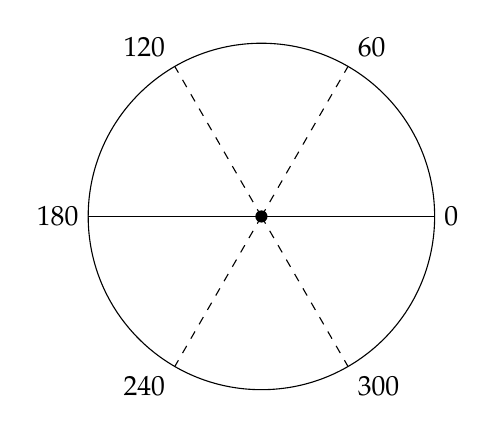
\begin{tikzpicture}[scale=2.2]
\coordinate (origin) at (0,0);
% Draw circle
\draw (origin) circle [radius=1];
% Draw axes
\draw (-1,0) node [left] {$180$} -- (1,0) node [right] {$0$};
%\draw (0,-1) node [below] {$270$} -- (0,1) node [above] {$90$};
% Draw other angles
\draw[dashed] (origin) -- +(60:1) node[above right] {$60$};
\draw[dashed] (origin) -- +(120:1) node[above left] {$120$};
\draw[dashed] (origin) -- +(240:1) node[below left] {$240$};
\draw[dashed] (origin) -- +(300:1) node[below right] {$300$};
% Dot at origin
\fill (origin) circle [radius=1pt];
\end{tikzpicture}
\hspace{5em}
% The unit circle divided into 30 degree segments
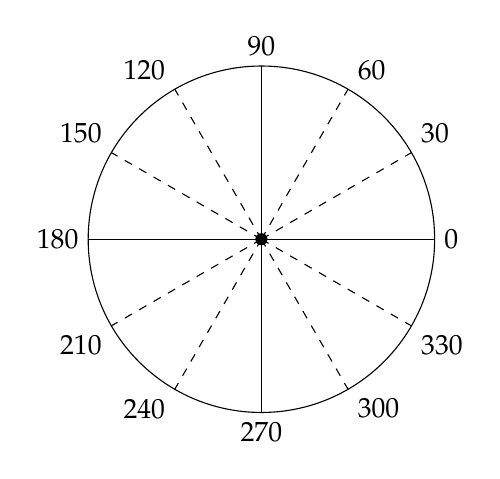
\begin{tikzpicture}[scale=2.2,baseline=-70pt]
\coordinate (origin) at (0,0);
% Draw circle
\draw (origin) circle [radius=1];
% Draw axes
\draw (-1,0) node [left] {$180$} -- (1,0) node [right] {$0$};
\draw (0,-1) node [below] {$270$} -- (0,1) node [above] {$90$};
% Draw other angles
\draw[dashed] (origin) -- +(30:1) node[above right] {$30$};
\draw[dashed] (origin) -- +(60:1) node[above right] {$60$};
\draw[dashed] (origin) -- +(120:1) node[above left] {$120$};
\draw[dashed] (origin) -- +(150:1) node[above left] {$150$};
\draw[dashed] (origin) -- +(210:1) node[below left] {$210$};
\draw[dashed] (origin) -- +(240:1) node[below left] {$240$};
\draw[dashed] (origin) -- +(300:1) node[below right] {$300$};
\draw[dashed] (origin) -- +(330:1) node[below right] {$330$};
% Dot at origin
\fill (origin) circle [radius=1pt];
\end{tikzpicture}
\end{center}
In radians:
\begin{center}
% The unit circle with radians divided into pi/3 segments
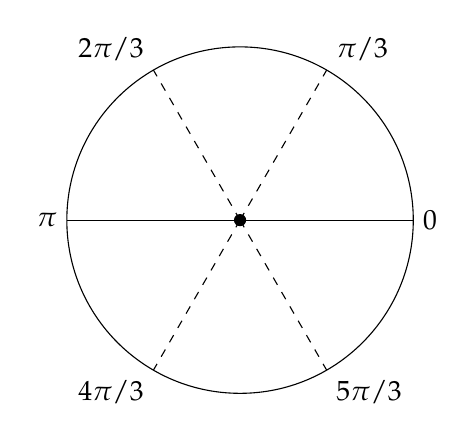
\begin{tikzpicture}[scale=2.2]
\coordinate (origin) at (0,0);
% Draw circle
\draw (origin) circle [radius=1];
% Draw axes
\draw (-1,0) node [left] {$\pi$} -- (1,0) node [right] {$0$};
% Draw other angles
\draw[dashed] (origin) -- +(60:1) node[above right] {$\pi/3$};
\draw[dashed] (origin) -- +(120:1) node[above left] {$2\pi/3$};
\draw[dashed] (origin) -- +(240:1) node[below left] {$4\pi/3$};
\draw[dashed] (origin) -- +(300:1) node[below right] {$5\pi/3$};
% Dot at origin
\fill (origin) circle [radius=1pt];
\end{tikzpicture}
\hspace{4em}
% The unit circle with radians divided into pi/6 segments
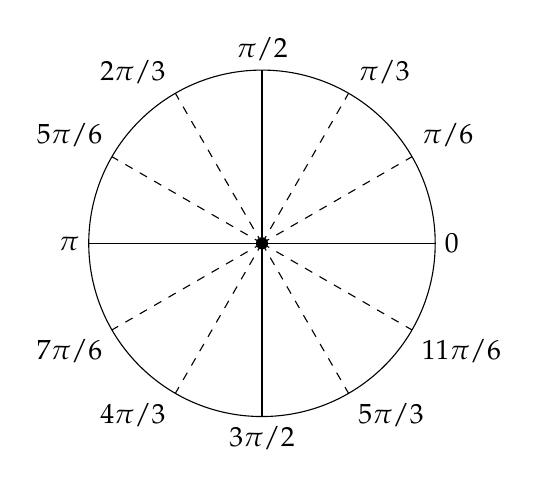
\begin{tikzpicture}[scale=2.2,baseline=-71pt]
\coordinate (origin) at (0,0);
% Draw circle
\draw (origin) circle [radius=1];
% Draw axes
\draw (-1,0) node [left] {$\pi$} -- (1,0) node [right] {$0$};
\draw (0,-1) node [below] {$3\pi/2$} -- (0,1) node [above] {$\pi/2$};
% Draw other angles
\draw[dashed] (origin) -- +(30:1) node[above right] {$\pi/6$};
\draw[dashed] (origin) -- +(60:1) node[above right] {$\pi/3$};
\draw[dashed] (origin) -- +(120:1) node[above left] {$2\pi/3$};
\draw[dashed] (origin) -- +(150:1) node[above left] {$5\pi/6$};
\draw[dashed] (origin) -- +(210:1) node[below left] {$7\pi/6$};
\draw[dashed] (origin) -- +(240:1) node[below left] {$4\pi/3$};
\draw[dashed] (origin) -- +(300:1) node[below right] {$5\pi/3$};
\draw[dashed] (origin) -- +(330:1) node[below right] {$11\pi/6$};
% Dot at origin
\fill (origin) circle [radius=1pt];
\end{tikzpicture}
\end{center}

Let us first compute the sine of $30^\circ$. In the right triangle:
\begin{center}
% Right triangle with 30 and 60 degree angles
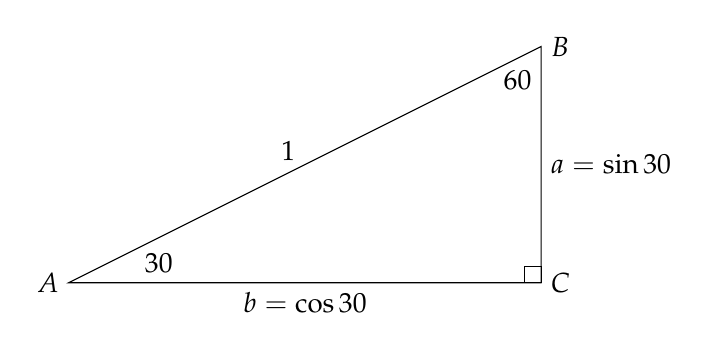
\begin{tikzpicture}[scale=6]
% Coordinates
\coordinate (origin) at (0,0);
\coordinate (lower-right) at (1,0);
\coordinate (upper-right) at (1,.5);
% Draw triangle
\draw (origin)
  node[left] {$A$} node[above right,xshift=24pt] {$30$} --
  node[below] {$b=\cos 30$} (lower-right) node[right] {$C$} --
  node[right] {$a=\sin 30$} (upper-right)
    node[right] {$B$} node[below left,yshift=-5pt] {$60$} --
  node[left,yshift=5pt] {$1$} cycle;
% Square for right angle
\draw (lower-right) rectangle +(-1pt,1pt);
\end{tikzpicture}
\end{center}
draw a line from $C$ to the hypotenuse that makes an angle of $30^\circ$ with the line $AC$:
\begin{center}
% Right triangle with 30 and 60 degree angles
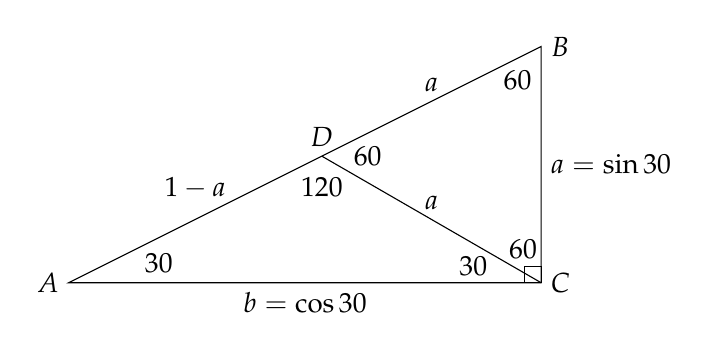
\begin{tikzpicture}[scale=6]
% Coordinates
\coordinate (origin) at (0,0);
\coordinate (lower-right) at (1,0);
\coordinate (upper-right) at (1,.5);
% Draw triangle
\draw (origin)
  node[left] {$A$} node[above right,xshift=24pt] {$30$} --
  node[below] {$b=\cos 30$} (lower-right) node[right] {$C$} --
  node[right] {$a=\sin 30$} (upper-right)
  node[right] {$B$} node[below left,yshift=-5pt] {$60$} --
  cycle;
% Get intersection of hypotenuse with line at 30 degrees
\path[name path=hypotenuse] (origin) -- (upper-right);
\path[name path=to-hyp] (lower-right) -- +(150:6mm);
\path[name intersections={of=hypotenuse and to-hyp,by=on-hyp}];
% Draw the line and label the angles
\draw (lower-right) 
    node[above left,yshift=5pt,xshift=2pt] {$60$}
    node [left,yshift=6pt,xshift=-16pt] {$30$} --
    (on-hyp)
    node[right,xshift=8pt] {$60$}
    node[below,yshift=-4pt] {$120$}
    node[above] {$D$};
% Label line segments
\path (lower-right) -- node[above] {$a$} (on-hyp);
\path (on-hyp) -- node[above] {$a$} (upper-right);
\path (origin) -- node[above,yshift=4pt] {$1-a$} (on-hyp);
% Square for right angle
\draw (lower-right) rectangle +(-1pt,1pt);
\end{tikzpicture}
\end{center}
Using various geometric facts about the angles in a triangle, we have inferred the other angles in the figure. Since $\triangle BCD$ is equilateral, all its sides are equal to $a=\sin 30$. Recall that $AB=1$ since we are in the unit circle, so $DA=1-a$. Since $\triangle ACD$ is isoceles, $a=1-a$. Therefore:
\begin{eqnarray*}
\sin 30 &=& a = 1-a\\
&=& \frac{1}{2}\,.
\end{eqnarray*}
From $\sin^2\theta + \cos^2\theta = 1$, we obtain:
\[
\cos 30 = \sqrt{1-\sin^2 30} = \sqrt{1-\left(\frac{1}{2}\right)^2} = \sqrt{\frac{3}{4}} = \frac{\sqrt{3}}{2}\,.
\]

%%%%%%%%%%%%%%%%%%%%%%%%%%%%%%%%%%%%%%%%%%%%%%%%%%%%%%%%%%%%%%%

\section{The sine and cosine of $(90-\theta)$}

Let us now turn to the computation of the sine and cosine of $60^\circ$. Since $60 = 90 - 30$, we suspect that there might be a simple relation between the trigonometric functions of $60^\circ$ and $30^\circ$. This becomes clear when we draw an angle of $90-\theta$ in the unit circle:
\begin{center}
% Quadrant with angle 90 - theta
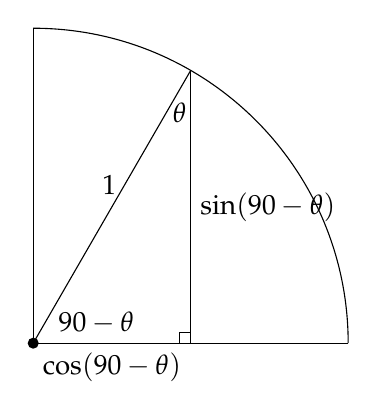
\begin{tikzpicture}[scale=4]
\coordinate (origin) at (0,0);
% Draw arc
\draw[name path=arc] (1,0) arc [start angle=0, end angle=90, radius=1];
% Draw x-axis
\draw[name path=x] (origin) -- (1,0);
% Draw y-axis
\draw (origin) -- (0,1);
% Draw ray
\draw[rotate=60,name path=ray] (origin) node [above right,xshift=2mm] {$90-\theta$} -- node [above,yshift=1pt,xshift=-1pt] {$1$} (1,0);
% Get intersection of arc and ray
\path [name intersections={of=ray and arc, by=on-circle}];
% Draw altitude from intersection to x-axis
\draw[name path=altitude] (on-circle) node[below,yshift=-8pt,xshift=-4pt] {$\theta$} -- node [right] {$\sin (90-\theta)$} (on-circle |- origin);
% Get intersection of altitude and x-axis
\path [name intersections={of=altitude and x, by=on-x}] (origin) -- node [below] {$\cos (90-\theta)$} (on-x);
% Square for right angle at intersection
\draw (on-x) rectangle +(-1pt,1pt);
% Dot at origin
\fill (origin) circle [radius=.5pt];
\end{tikzpicture}
\end{center}
Since the angle where the triangle intersects the unit circle is $\theta$, the trigonometric functions of $90-\theta$ can be obtained from those of $\theta$ by switching ``opposite'' and ``adjacent'':
\begin{eqnarray*}
\cos (90-\theta) &=& \sin \theta\\
\sin (90-\theta) &=& \cos \theta\,.
\end{eqnarray*}
Another way of seeing this is to note that the triangle is congruent to the triangle we used to compute $\sin\theta$ and $\cos \theta$:
\begin{center}
% Quadrant with angles 90 and 90 - theta
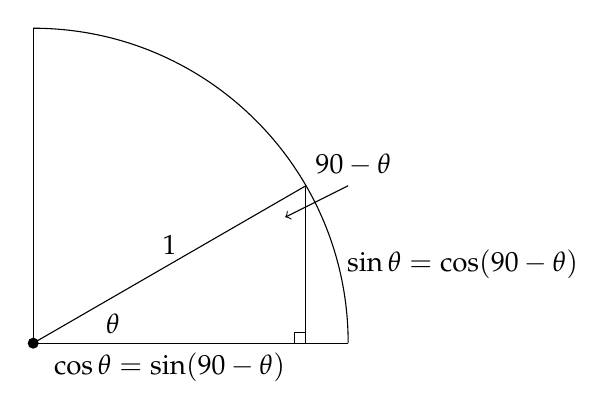
\begin{tikzpicture}[scale=4]
\coordinate (origin) at (0,0);
% Draw arc
\draw[name path=arc] (1,0) arc [start angle=0, end angle=90, radius=1];
% Draw x-axis
\draw[name path=x] (origin) -- (1,0);
% Draw y-axis
\draw (origin) -- (0,1);
% Draw ray
\draw[rotate=30,name path=ray] (origin) node [above right,xshift=8mm] {$\theta$} -- node [above] {$1$} (1,0);
% Get intersection of arc and ray
\path [name intersections={of=ray and arc, by=on-circle}];
% Draw altitude from intersection to x-axis
\draw[name path=altitude] (on-circle) node [above right] {$90-\theta$} -- node [right,xshift=4mm] {$\sin \theta = \cos (90-\theta)$} (on-circle |- origin);
% Arrow from label
\draw[->] (1,.5) -- +(-.2,-.1);
% Get intersection of altitude and x-axis
\path [name intersections={of=altitude and x, by=on-x}] (origin) -- node [below] {$\cos \theta = \sin (90-\theta)$} (on-x);
% Square for right angle at intersection
\draw (on-x) rectangle +(-1pt,1pt);
\fill (origin) circle [radius=.5pt];
\end{tikzpicture}
\end{center}
It follows that:
\[
\renewcommand{\arraystretch}{1.3}
\begin{array}{l}
\cos 60 = \cos (90-30) = \sin 30 = \displaystyle \frac{1}{2}\\
\sin 60 = \sin (90-30) = \cos 30 = \displaystyle \frac{\sqrt{3}}{2}\,.
\end{array}
\]
The trigonometric functions for multiples of $30^\circ$, $60^\circ$ can be easily computed by examining the unit circle:

\begin{displaymath}
\renewcommand{\arraystretch}{1.3}
\begin{array}{|c|c|c|c|}
\hline
\textrm{Angle} & \textrm{Angle} & \sin & \cos\\
\textrm{(degrees)} & \textrm{(radians)} & & \\\hline
0&0&0&1\\\hline
30& \pi/6&  1/2 &  \sqrt{3}/2 \\\hline
60& \pi/3&  \sqrt{3}/2 &  1/2 \\\hline
90&\pi/2&1&0\\\hline
120& 2\pi/3&  \sqrt{3}/2 &  -1/2\\\hline
150& 5\pi/6&  1/2 &  -\sqrt{3}/2\\\hline
180&\pi&0&-1\\\hline
210& 7\pi/6&  -1/2 &  -\sqrt{3}/2\\\hline
240& 4\pi/3&  -\sqrt{3}/2 &  -1/2\\\hline
270&3\pi/2&-1&0\\\hline
300& 5\pi/3&  -\sqrt{3}/2 &  1/2\\\hline
330& 11\pi/6&  -1/2 &  \sqrt{3}/2\\
\hline
\end{array}
\end{displaymath}


%%%%%%%%%%%%%%%%%%%%%%%%%%%%%%%%%%%%%%%%%%%%%%%%%%%%%%%%%%%%%%%

\section{Multiple angle formulas}

Unfortunately, you have to memorize the formula for the sine of the sum of two angles:
\[
\sin(\alpha+\beta)=\sin\alpha\cos\beta+\cos\alpha\sin\beta\,.
\]
The proof is not hard but it is difficult to reproduce on a moment's notice. The other formulas follow easily. The sine of the difference of two angles is:
\[
\sin(\alpha-\beta)=\sin(\alpha+(-\beta))=\sin\alpha\cos(-\beta)+\cos\alpha\sin(-\beta) = 
\sin\alpha\cos\beta-\cos\alpha\sin\beta\,.
\]
For the cosine:
\begin{eqnarray*}
\cos(\alpha+\beta)&=&\sin(90-(\alpha+\beta))\\
&=& \sin((90-\alpha)-\beta)\\
&=& \sin(90-\alpha)\cos\beta-\cos(90-\alpha)\sin\beta\\
&=&\cos\alpha\cos\beta - \sin\alpha\sin\beta\,,
\end{eqnarray*}
and:
\[
\cos(\alpha-\beta) = \cos\alpha\cos(-\beta) - \sin\alpha\sin(-\beta) = 
\cos\alpha\cos\beta + \sin\alpha\sin\beta\,.
\]

The double angle formulas follow from the formulas for the sum of two angles:
\begin{eqnarray*}
\sin 2\alpha &=& \sin(\alpha+\alpha)\\
&=& \sin\alpha\cos\alpha+\cos\alpha\sin\alpha\\
&=& 2\sin\alpha\cos\alpha\\
\cos 2\alpha &=& \cos(\alpha+\alpha)\\
&=& \cos\alpha\cos\alpha - \sin\alpha\sin\alpha\\
&=& \cos^2\alpha-\sin^2\alpha\\
&=& \cos^2\alpha- (1-\cos^2\alpha)\\
&=& 2\cos^2\alpha-1\\
\cos 2\alpha &=& \cos^2\alpha-\sin^2\alpha\\
&=& (1-\sin^2\alpha) -\sin^2\alpha\\
&=&  1-2\sin^2\alpha\,.
\end{eqnarray*}

%%%%%%%%%%%%%%%%%%%%%%%%%%%%%%%%%%%%%%%%%%%%%%%%%%%%%%%%%%%%%%%

\section{Summary}

We started from the definition of the trigonometric functions sine and cosine in terms of the ratios of the sides of a right triangle. Since the absolute values of the sides do not matter, we took the hypotenuse to be $1$. From Pythagoras's theorem:
\[
\sin^2 \theta + \cos^2\theta = 1\,
\]
and:
\[
\sin 45 = \cos 45 = \frac{\sqrt{2}}{2}\,.
\]
Using an elementary construction and geometric facts about triangles, we showed that:
\[
\renewcommand{\arraystretch}{1.3}
\begin{array}{l}
\sin 30 = \cos 60 = \frac{1}{2}\\
\cos 30 = \sin 60 = \frac{\sqrt{3}}{2}\,.
\end{array}
\]
Given the sine and cosine of any angle $\theta$ in the first quadrant, our friend the unit circle enabled us to immediately compute the trigonometric functions of any angle obtained from $\theta$ by adding or subtracting multiples of $90^\circ$. In particular, we know the sine and cosine of the following angles:
\begin{center}
% The unit circle with degrees
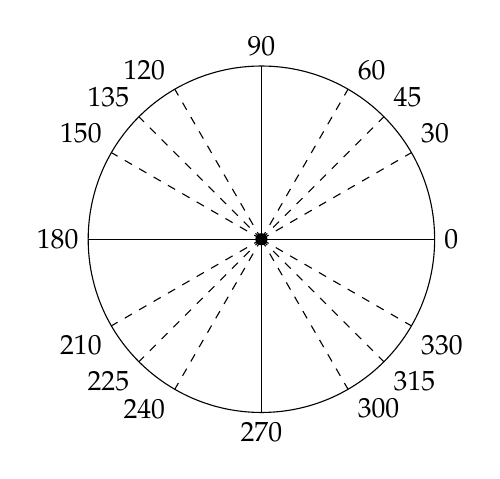
\begin{tikzpicture}[scale=2.2]
\coordinate (origin) at (0,0);
% Draw circle
\draw (origin) circle [radius=1];
% Draw axes
\draw (-1,0) node [left] {$180$} -- (1,0) node [right] {$0$};
\draw (0,-1) node [below] {$270$} -- (0,1) node [above] {$90$};
% Draw other angles
\draw[dashed] (origin) -- +(30:1) node[above right] {$30$};
\draw[dashed] (origin) -- +(45:1) node[above right] {$45$};
\draw[dashed] (origin) -- +(60:1) node[above right] {$60$};
\draw[dashed] (origin) -- +(120:1) node[above left] {$120$};
\draw[dashed] (origin) -- +(135:1) node[above left] {$135$};
\draw[dashed] (origin) -- +(150:1) node[above left] {$150$};
\draw[dashed] (origin) -- +(210:1) node[below left] {$210$};
\draw[dashed] (origin) -- +(225:1) node[below left] {$225$};
\draw[dashed] (origin) -- +(240:1) node[below left] {$240$};
\draw[dashed] (origin) -- +(300:1) node[below right] {$300$};
\draw[dashed] (origin) -- +(315:1) node[below right] {$315$};
\draw[dashed] (origin) -- +(330:1) node[below right] {$330$};
% Dot at origin
\fill (origin) circle [radius=1pt];
\end{tikzpicture}
\hfil
% The unit circle with radians
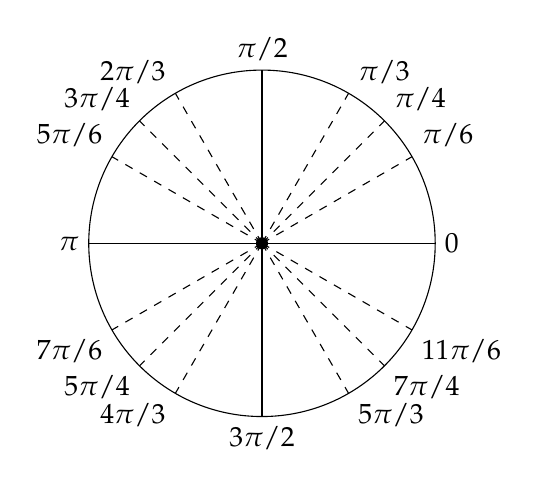
\begin{tikzpicture}[scale=2.2]
\coordinate (origin) at (0,0);
% Draw circle
\draw (origin) circle [radius=1];
% Draw axes
\draw (-1,0) node [left] {$\pi$} -- (1,0) node [right] {$0$};
\draw (0,-1) node [below] {$3\pi/2$} -- (0,1) node [above] {$\pi/2$};
% Draw other angles
\draw[dashed] (origin) -- +(30:1) node[above right] {$\pi/6$};
\draw[dashed] (origin) -- +(45:1) node[above right] {$\pi/4$};
\draw[dashed] (origin) -- +(60:1) node[above right] {$\pi/3$};
\draw[dashed] (origin) -- +(120:1) node[above left] {$2\pi/3$};
\draw[dashed] (origin) -- +(135:1) node[above left] {$3\pi/4$};
\draw[dashed] (origin) -- +(150:1) node[above left] {$5\pi/6$};
\draw[dashed] (origin) -- +(210:1) node[below left] {$7\pi/6$};
\draw[dashed] (origin) -- +(225:1) node[below left] {$5\pi/4$};
\draw[dashed] (origin) -- +(240:1) node[below left] {$4\pi/3$};
\draw[dashed] (origin) -- +(300:1) node[below right] {$5\pi/3$};
\draw[dashed] (origin) -- +(315:1) node[below right] {$7\pi/4$};
\draw[dashed] (origin) -- +(330:1) node[below right] {$11\pi/6$};
% Dot at origin
\fill (origin) circle [radius=1pt];
\end{tikzpicture}
\end{center}

\bigskip

\textbf{\large All this without memorizing anything except the definitions of sine and cosine!}

\bigskip

The formulas for multiple angles are easily derived from the formulas for $\sin(\alpha+\beta)$, but you will have to memorize that one formula because it is not easy to derive.

%%%%%%%%%%%%%%%%%%%%%%%%%%%%%%%%%%%%%%%%%%%%%%%%%%%%%%%%%%%%%%%
\newpage

\appendix

\section{The law of sines}

The law of sines is not difficult to memorize, but it is worthwhile to see how easily it can be derived. Given a triangle $\triangle ABC$, drop an altitude from one vertex:
\begin{center}
% Law of sines
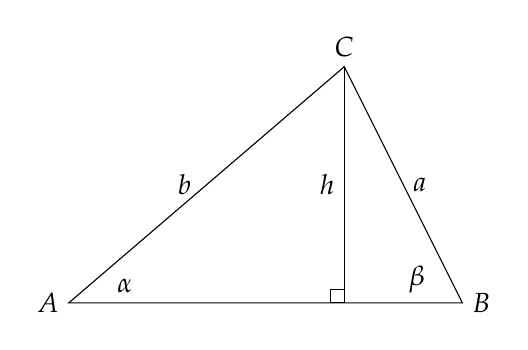
\begin{tikzpicture}[scale=5]
% Coordinates
\coordinate (a) at (0,0);
\coordinate (b) at (1,0);
\coordinate (c) at (.7,.6);
% Draw triangle
\draw (a) node[left]  {$A$} node[above right,xshift=14pt] {$\alpha$} --
      (b) node[right] {$B$} node[above left,xshift=-10pt] {$\beta$} --
          node[right] {$a$}
      (c) node[above] {$C$} --
          node[left,xshift=-2pt]  {$b$}
      cycle;
\draw (c) -- node[left] {$h$} (c |- b);
\draw (c |- b) rectangle +(-1pt,1pt);
\end{tikzpicture}
\end{center}
Since:
\begin{eqnarray*}
\sin\alpha &=& \frac{h}{b}\\
\sin\beta &=& \frac{h}{a}\,,
\end{eqnarray*}
we have:
\begin{eqnarray*}
b\sin\alpha &=& a\sin\beta\\
\frac{\sin\alpha}{a} &=& \frac{\sin\beta}{b}\,.
\end{eqnarray*}

A similar construction gives the equality of these ratios with $\displaystyle\frac{\sin\gamma}{c}$.

%%%%%%%%%%%%%%%%%%%%%%%%%%%%%%%%%%%%%%%%%%%%%%%%%%%%%%%%%%%%%%%

\section{The law of sines in a circle}

There is an alternate proof of the law of sines that also relates the ratios of the sines to the sides of the triangle to the radius of a circumscribed circle.\footnote{I would like to thank Avital Elbaum Cohen for bringing this proof to my attention.}

Consider the triangle $\triangle ABC$ and its circumscribed circle.\footnote{This proof is for an acute triangle. The proof for an obtuse triangle is similar.} (Every triangle can be circumscribed by a circle whose center is the intersection of the perpendicular bisectors of its sides.) Find the point $D$ on the circle such that $DB$ passes through the center of the circle. Draw the line $AD$:

% Angles subtending the same chord are equal
%
\begin{center}
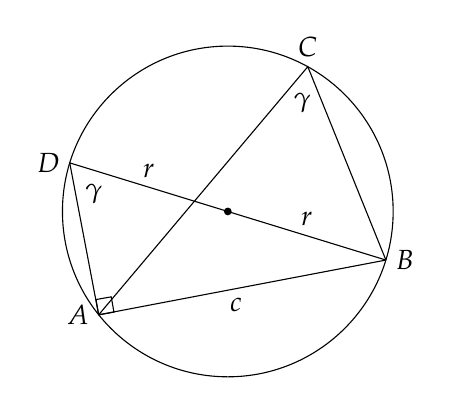
\begin{tikzpicture}[scale=.7]
% Draw the circle at the origin
\coordinate (origin) at (0,0);
\draw [name path=circle] (origin) circle [radius=3];
% Define a path that intersects the circle
\coordinate (a) at (-3,-2);
\coordinate (b) at (3.3,-.8);
\path [name path=chord] (a) -- node [below] {$c$} (b);
% Get the intersections and draw the chord
\path [name intersections={of=circle and chord,by={i1,i2}}];
\draw (i1) node [left] {$A$} -- (i2) node [right] {$B$};
% Define a path to the third vertex and get the intersection
\coordinate (c) at (1.3,3);
\path [name path=side] (i2) -- (c);
\path [name intersections={of=circle and side,by={i3,i4}}];
% Draw the other two sides of the triangle
\draw (i2) -- (i3) node [above] {$C$} node [below,xshift=-2pt,yshift=-6pt] {$\gamma$} -- (i1);
% Define a path through the origin and get its intersection with the circle
\path [name path=diameter] (i2) -- ($ (i2) ! 2.2 ! (origin) $);
\path [name intersections={of=circle and diameter,by={i5,i6}}];
% Draw the triangle subtending the diameter
\draw (i2) -- (i5) node [left] {$D$} node [below right,xshift=2pt,yshift=-4pt] {$\gamma$} -- (i1);
\path (i2) -- node [above] {$r$} ($(i2)!.5!(i5)$) -- node [above] {$r$} (i5);
% Dot at origin
\fill (origin) circle (2pt);
% Draw small square
\draw [rotate=10] (i1) rectangle +(8pt,8pt);
\end{tikzpicture}
\end{center}

Since $\angle ADB$ and $\angle ACB$ subtend the same chord $AB$, they are equal. Since $\angle DAB$ subtends a diameter it is equal to $90^\circ$. Therefore:
\[
\sin\gamma = \displaystyle \frac{c}{2r}\,.
\]
A similar construction can be done for the other vertices of the triangle giving:
\[
\frac{1}{2r} = \frac{\sin\gamma}{c} = \frac{\sin\beta}{b} = \frac{\sin\alpha}{a}\,.
\]

%%%%%%%%%%%%%%%%%%%%%%%%%%%%%%%%%%%%%%%%%%%%%%%%%%%%%%%%%%%%%%%

\section{The law of cosines}

The law of cosines is also not hard to memorize and its proof is not obvious. Nevertheless, we give a proof to show that only geometric facts and the definitions of sine and cosine are needed.\footnote{This proof is for an acute triangle. The proof for an obtuse triangle is similar.} Drop an altitude from one vertex:
\begin{center}
% Law of cosines for acute triangle
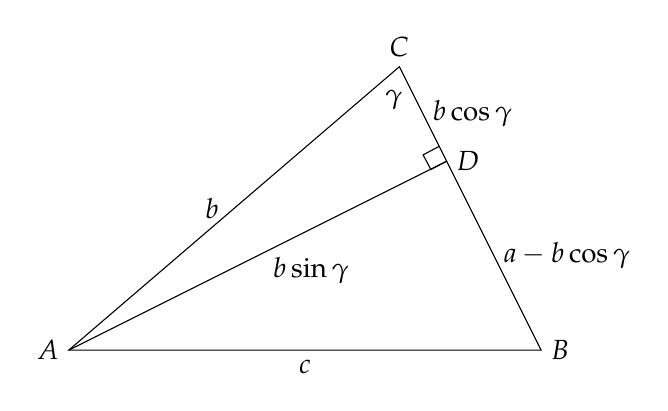
\begin{tikzpicture}[scale=6]
% Coordinates
\coordinate (a) at (0,0);
\coordinate (b) at (1,0);
\coordinate (c) at (.7,.6);
% Draw triangle
\draw (a) node[left]  {$A$} --
          node[below] {$c$}
      (b) node[right] {$B$} --
      (c) node[above] {$C$} node[below,yshift=-5pt,xshift=-2pt] {$\gamma$} --
          node[left,xshift=-2pt]  {$b$}
      cycle;
\draw (a) -- node[below right,yshift=3pt,xshift=2pt] {$b\sin\gamma$} ($(b)!(a)!(c)$);
\draw[rotate=118] ($(b)!(a)!(c)$) -- ++(0,1pt) -- ++(1pt,0) -- ++(0,-1.1pt);
\path (c) -- node[right] {$b\cos\gamma$} ($(b)!(a)!(c)$) node[right] {$D$};
\path ($(b)!(a)!(c)$) -- node[right] {$a-b\cos\gamma$} (b);
\end{tikzpicture}
\end{center}
In the right triangle $\triangle ADC$, the hypotenuse is $b$ and we can compute the lengths of the other two sides by trigonometry. The length of $DB$ is the length of $CB$ ($a$, not denoted in the diagram) minus the length of $CD$ which we just computed. Using Pythagoras's theorem on the triangle $\triangle ABD$:
\begin{eqnarray*}
c^2 &=& (a-b\cos\gamma)^2 + b^2\sin^2\gamma\\
&=& a^2-2ab\cos\gamma + b^2\cos^2\gamma + b^2\sin^2\gamma\\
&=& a^2-2ab\cos\gamma + b^2(\cos^2\gamma + \sin^2\gamma)\\
&=& a^2+b^2-2ab\cos\gamma\,.
\end{eqnarray*}
Pythagoras's theorem is obtained by setting $\gamma=90^\circ$, so we see that the law of cosines is a generalization of Pythagoras's theorem.

%%%%%%%%%%%%%%%%%%%%%%%%%%%%%%%%%%%%%%%%%%%%%%%%%%%%%%%%%%%%%%%

\newpage

\section{The area of a triangle}

The same construction:
\begin{center}
% Area of a triangle
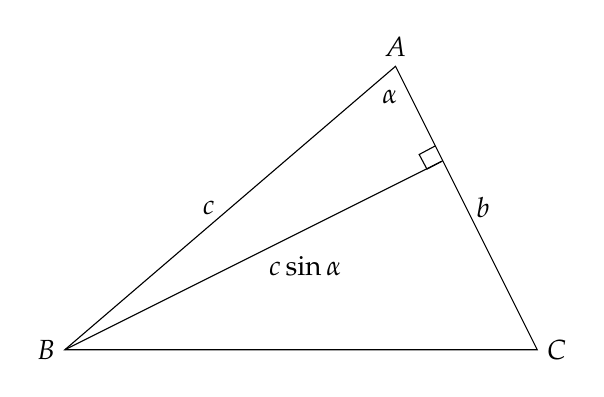
\begin{tikzpicture}[scale=6]
% Coordinates
\coordinate (a) at (0,0);
\coordinate (b) at (1,0);
\coordinate (c) at (.7,.6);
% Draw triangle
\draw (a) node[left]  {$B$} --
%          node[below] {$c$}
      (b) node[right] {$C$} --
      (c) node[above] {$A$} node[below,yshift=-5pt,xshift=-2pt] {$\alpha$} --
          node[left,xshift=-2pt]  {$c$}
      cycle;
\draw (a) -- node[below right,yshift=3pt,xshift=2pt] {$c\sin\alpha$} ($(b)!(a)!(c)$);
\draw[rotate=118] ($(b)!(a)!(c)$) -- ++(0,1pt) -- ++(1pt,0) -- ++(0,-1.1pt);
\path (c) -- ($(b)!(a)!(c)$);
\path (b) -- node[right] {$b$} (c);
\end{tikzpicture}
\end{center}
gives the generalized formula for the area of a triangle:
\[
S(\triangle ABC) = \frac{1}{2}\cdot\textit{base}\cdot\textit{height} = \frac{1}{2}bc\sin\alpha\,.
\]
If $\alpha$ is a right angle, $S(\triangle ABC) = \frac{1}{2}bc$, as expected.

\end{document}
